\begin{savequote}[75mm]
What emerged from the darkness of the caves, from the depths of millennia, we wish to pass on to machines, in one brief circuit closure, to spark reason into existence.
\qauthor{Stanisław Lem}
\end{savequote}


\chapter{Machine Learning }
\label{chap:ml}

Although machine learning experienced rapid growth in the second decade of the new Millenium, it has come a long and difficult path to become almost omnipresent in everyone's life and in many scientific disciplines.
The high energy physics is not an exception, and in fact, the majority of this thesis describes various approaches to application of computational intelligence in field of particle physics.
This chapter contains an introduction to the machine learning methods used in further chapters.

One of the events that can be thought of as the birth of machine learning is the invention of the perceptron.
The perceptron was the protoplast of the artificial neural networks we know today. It was created by Frank Rosenblatt \cite{Rosenblatt1958ThePA} in 1958.
In essence, the perceptron is what we today can call a single layer neural network.
Famously, the over-promising of the capabilities of the perceptron was one of the leading causes for the so-called ``first AI winter''\cite{enwiki:1076647189}.
It was quickly discovered that the perceptron cannot be efficiently scaled to solve more generic problems and is, in particular, unable to solve the XOR task.
Although the concept of multi-layer perceptron was already proposed, it lacked a viable way of training the parameters.
This was later mitigated by the use of back-propagation as a method for training the parameters of the artificial neural networks.
Back-propagation was popularised in the 1980s. This also coincides with a time of significant growth in interest in artificial intelligence.
The primary trend was the usage of so-called ``expert systems'', which in reality were a set of predefined if-then statements built around expert knowledge.
% https://towardsdatascience.com/history-of-the-second-ai-winter-406f18789d45
Again, the hype for the AI and under-delivered solutions led to a cut in funding in research in this area and the ``second AI winter'', which lasted to about the second half of the first decade of the new Millenium.
The significant development in computing power and the increased ability to create vast training data-sets allowed for the dynamic growth of this field of computer science that we observe to this day.

% (@TODO maybe add hype lifecycle graphics here?)

% function that maps its input <math>\mathbf{x}</math> (a real-valued [[Vector space|vector]]) to an output value <math>f(\mathbf{x})</math> (a single [[Binary function|binary]] value):

% $$
% f(\mathbf{x}) = \begin{cases}1 & \text{if }\ \mathbf{w} \cdot \mathbf{x} + b > 0,\\0 & \text{otherwise}\end{cases}
% $$
\section{Areas of machine learning}

Machine learning can be divided into three general categories:
\begin{itemize}
\item \textbf{Supervised learning} expects pairs of desired input and output $(X,Y)$.
Supervised learning models assume that there exists a function $f$ where $y = f(x)$, and through its workings, tries to approximate the $f$ function.
This is by far most used type of machine learning algorithms, as given correct set of data, it is relatively easy to control the algorithms.
Problems that can provide input-output pairs of data also often allow assessing a model's performance with a single, easy-to-understand metric.

\item \textbf{Unsupervised learning} doesn't expect an exact output paired with given output. It does not expect output at all.
Generally, the tasks that are solved by unsupervised learning focus on discovering structures inside the data, like clusters and groups. There is a rising area of usage for the generation of the data points using the unknown inner distribution of the data.

\item \textbf{Reinforcement learning} usually focuses on the action taken in a given environment. Instead of the exact output matching the input, there is a defined reward that the reinforcement learning system is trying to maximise.

\end{itemize}
\section{Neural Networks}

Although the (artificial) neural networks are hardly the only machine learning technique available, they are the current go-to solutions for many  machine learning problems. This section will introduce the reader to the basics of modern neural network techniques, as they play a crucial role in the research discussed in the further chapters.

\begin{figure}
  \centering
  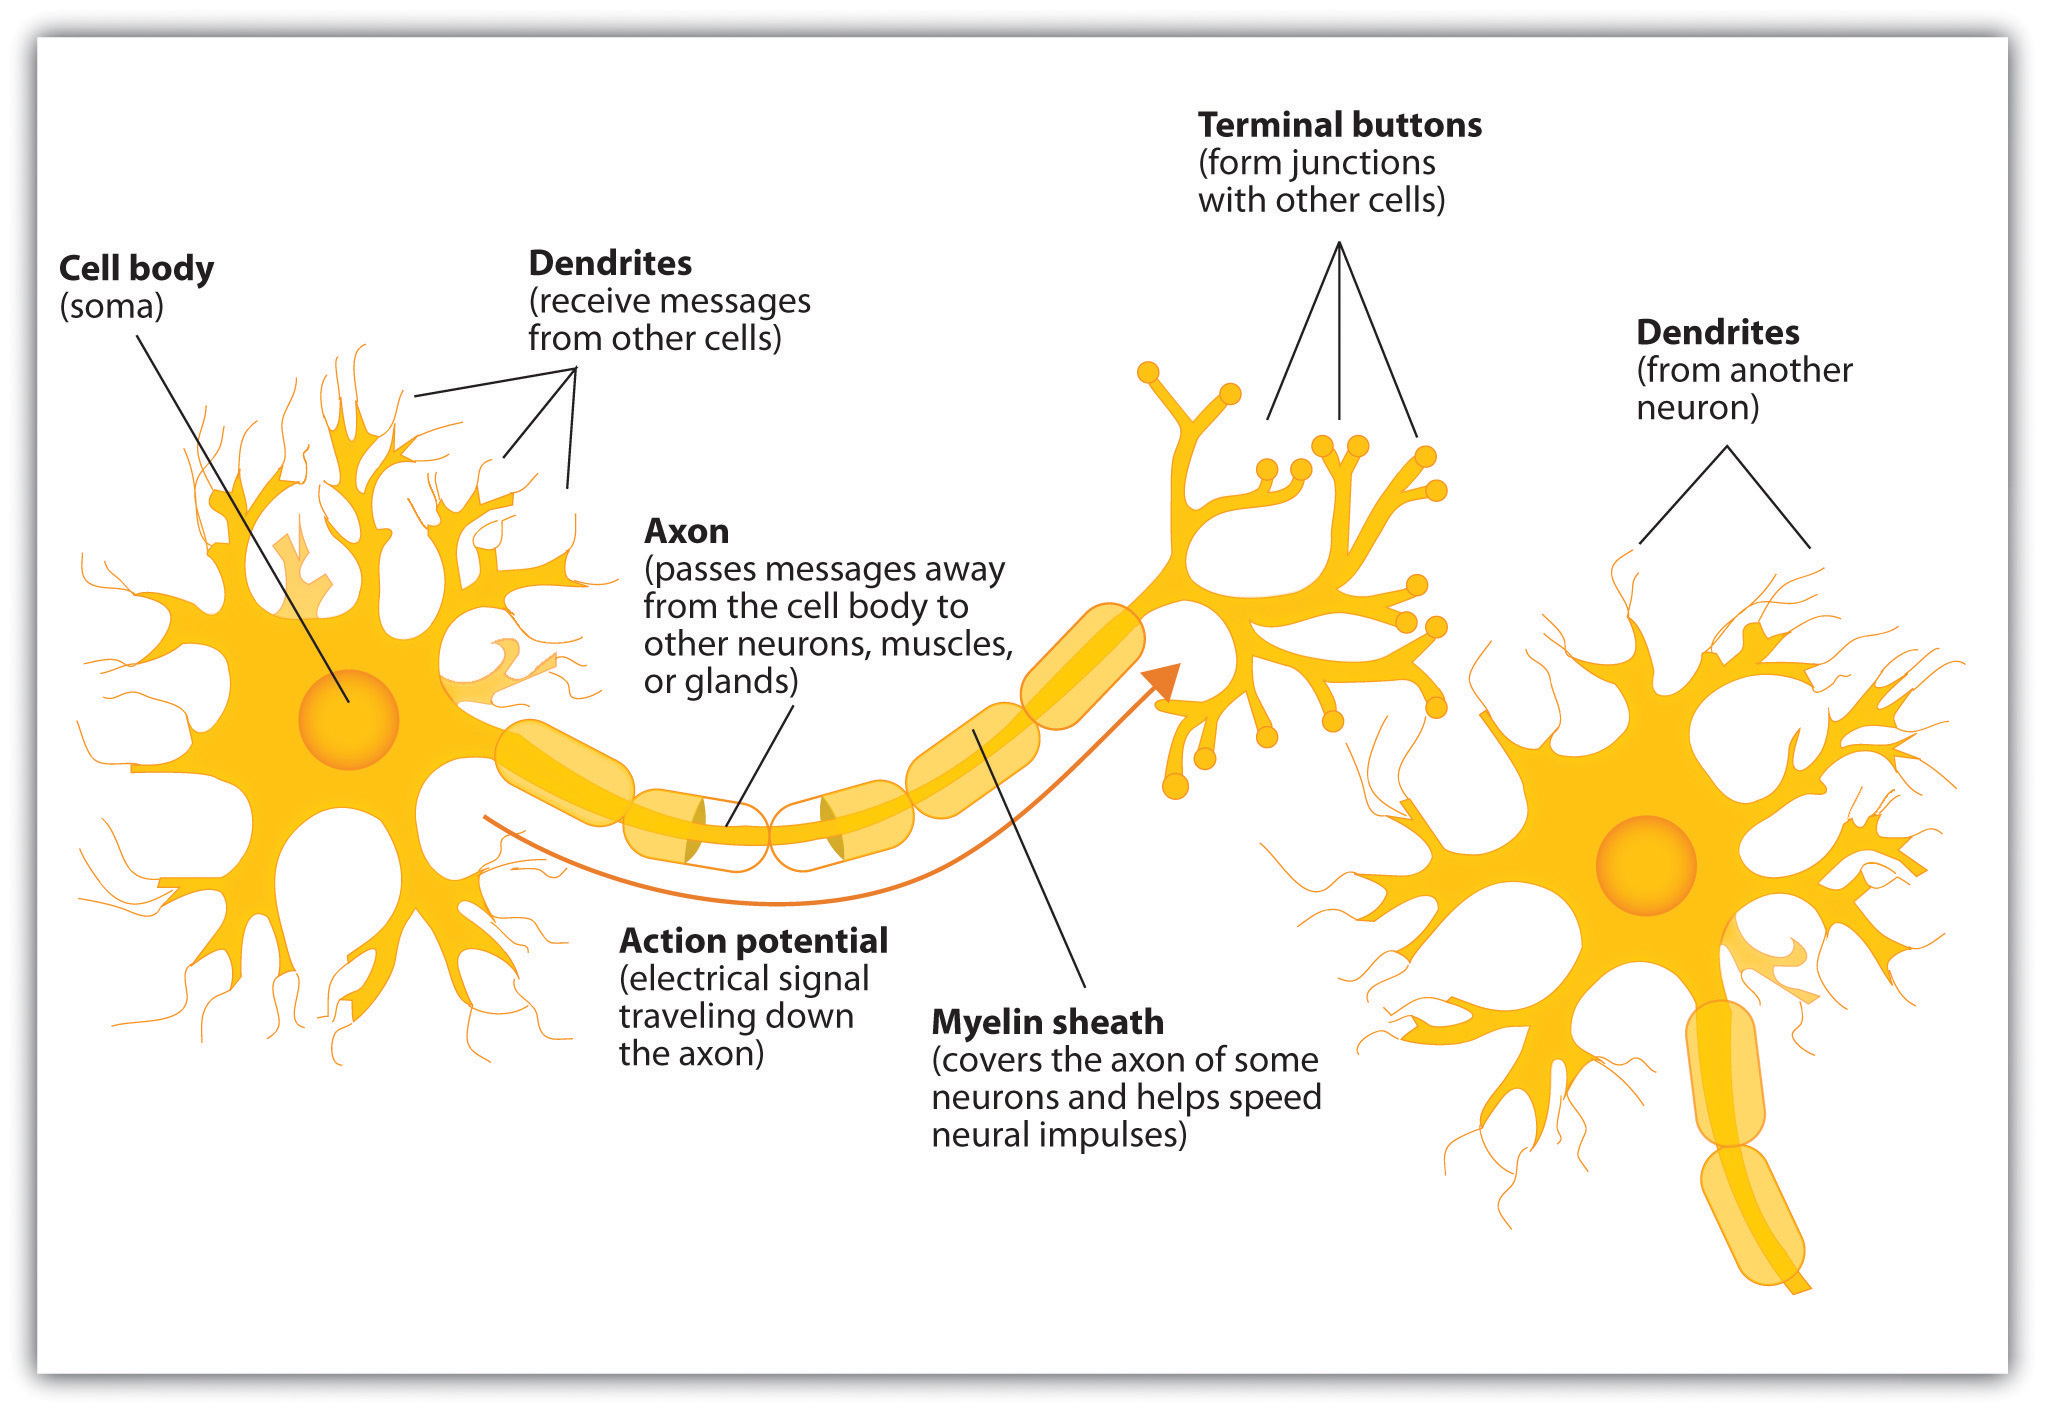
\includegraphics[width=0.7\linewidth]{figures/chapter3/Components_of_neuron.jpg}
  \caption[neron]{Components of the neuron\footnotemark. }
  \label{fig:real_neuron}
\end{figure}

\footnotetext{Source: \url{https://en.wikipedia.org/wiki/File:Components_of_neuron.jpg}}

\subsection{Multi-Layer Perceptron}

The artificial neural networks are based on a simplified model of the actual biological neural (nervous) tissue. 
A single neuron contains many dendrites and an axon, as visible in Fig. \ref{fig:real_neuron}.
The electrochemical potential supplied to the dendrites is accumulated, and then if a certain threshold is exceeded, the axon fires an electrochemical signal.
While it is true that this model of a neuron is a large oversimplification, the idea can be boiled down to the following mathematical formula:

\begin{align*}
f(x)=
\begin{cases}
    1,& \text{if } \sum_{i} x_{i} \geq T \\
    0,              & \text{otherwise}
\end{cases}
\end{align*}

The function above responds with 1 when the sum of the input signals $x_{i}$ is greater than threshold $T$.
This was extended by Rosenblat by addition of weights to the input and activation function.
The threshold can be represented as additional non-weighed input $b$.

\begin{align*}
f(x)=
\begin{cases}
    1,& \text{if } activation(\sum_{i} w_{i}x_{i} + b) \geq 0 \\
    0,              & \text{otherwise}
\end{cases}
\end{align*}

For binary classification, it may be useful to get the answer represented in the range between zero and one, which actually may be applied by using the activation function only in 0..1 domain, but other uses of neural networks may call for linear output (regression tasks).

\begin{align*}
f(x)= activation(\sum_{i} w_{i}x_{i} + b)
\end{align*}

\begin{figure}
  \centering
  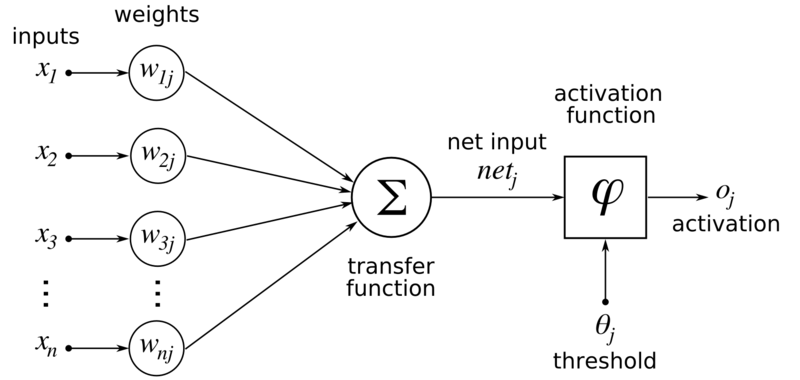
\includegraphics[width=0.7\linewidth]{figures/chapter3/ArtificialNeuronModel_english.png}
  \caption[singleann]{A visual, graph-based representation of a single artificial neural network neuron\footnotemark. }
  \label{fig:single_neuron}
\end{figure}

\footnotetext{Source \url{https://commons.wikimedia.org/wiki/File:ArtificialNeuronModel_english.png}}

This can be represented graphically as a simple graph with inputs and outputs (Fig. \ref{fig:single_neuron}).
Individual artificial neurons may be grouped in layers of neurons, sourcing the same inputs, as depicted on \ref{fig:multilayer_neuron}.
And this is where Multi-Layered Perceptron (MLP) got its name.
The forward pass in the neural network is the input undergoing multiplication with each layer of the network sequentially, and in effect, it produces the output.
The typical agreement in the ML community is that MLP is any simple neural network with arbitrary activation and with more than two layers.
To much of the disappointment of many computer science students, the difference between ``deep learning'' and MLP is commonly accepted to be with just a number of layers, with deep learning starting after two layers.

\begin{figure}
  \centering
  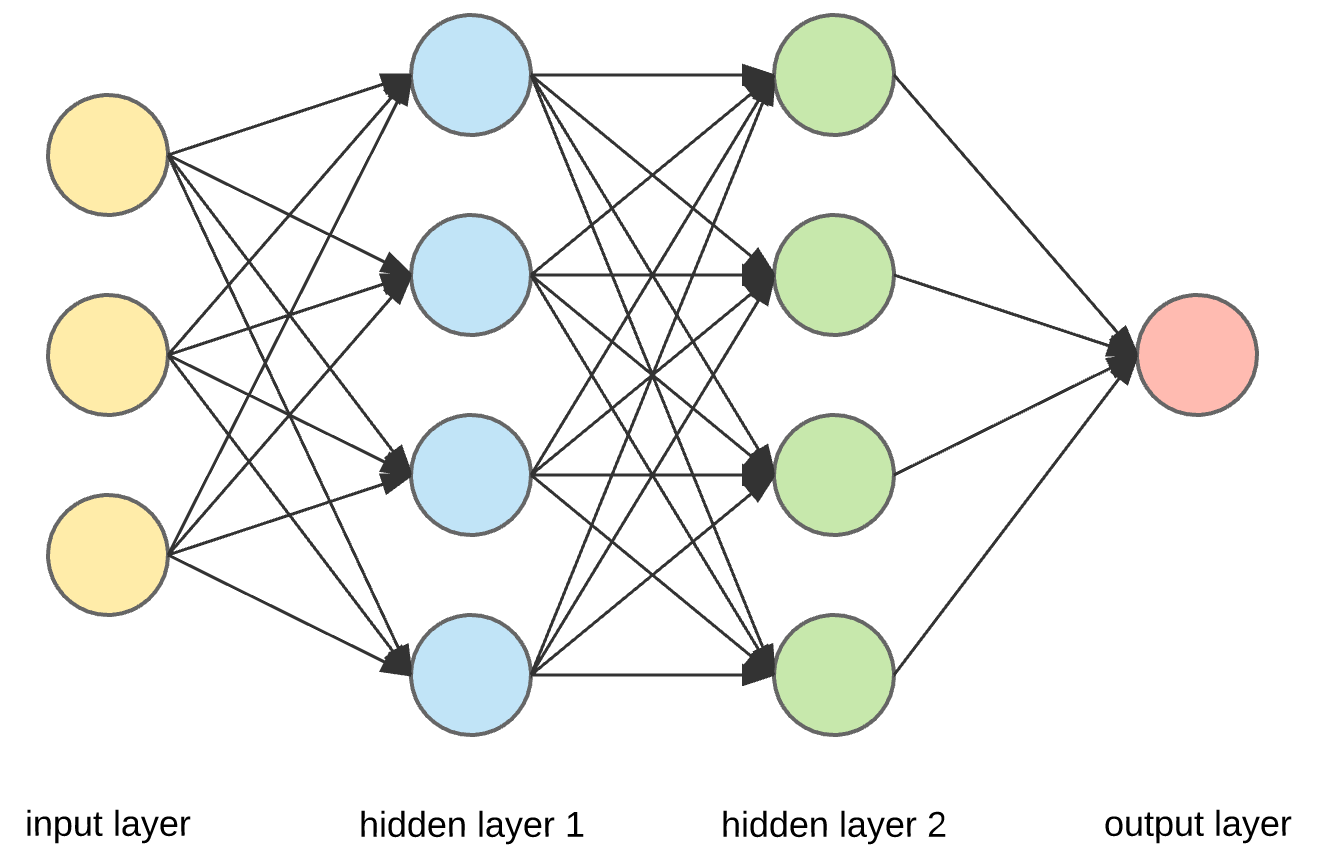
\includegraphics[width=0.5\linewidth]{figures/chapter3/1_3fA77_mLNiJTSgZFhYnU0Q.png}
  \caption[multilayer ann]{A graphical representation of multi-layer neural network\footnotemark. }
  \label{fig:multilayer_neuron}
\end{figure}
\footnotetext{Source

  \url{https://towardsdatascience.com/everything-you-need-to-know-about-neural-networks-and-backpropagation-machine-learning-made-easy-e5285bc2be3a}}

% https://towardsdatascience.com/multilayer-perceptron-explained-with-a-real-life-example-and-python-code-sentiment-analysis-cb408ee93141
% https://machinelearningmastery.com/neural-networks-crash-course/
% https://www.sciencedirect.com/topics/computer-science/multilayer-perceptron
\subsection{Stochastic gradient descent and Backpropagation}

The ``learning'' part of machine learning comes from the fact that the ``machine'' is given examples, pairs of input and desired output $(x,y)$.
The goal of the machine is to find such function $f(x)$ that $y=f(x)$.
Realistically speaking, not all of the tasks might be representable by the machine, so we expect approximation $y \approx f(x)$.
The error of this approximation can be expressed as $\epsilon = y - f(x)$.
Because a simple difference of two vectors may not be most suitable, we define a network's loss metric which is a function that given network output $f(x)$ and the target value $y$ will yield an error value $\epsilon = loss(f(x), y)$.
Several possible loss metrics exist, which can be used in a number of cases.
For classification, the popular loss metric is log-loss also known as cross-entropy, visible in Eq. \ref{eq:logloss} where $p$ is a predicted probability.
For regression tasks, an example of a loss metric is the mean squared error (MSE).

\begin{align}
 L_{\log}(y, p) = -(y \log (p) + (1 - y) \log (1 - p))
\label{eq:logloss}
\end{align}

The metrics can assess the quality of the output of the neural network.
This gives the opportunity to measure the error of the network, and in turn, we can optimise its response with respect to its weights.
The popular way of doing this is using a stochastic gradient descent which is a variation of a gradient descent algorithm.
The gradient descent algorithm is a minimisation algorithm that finds the optimal solution by following the gradient of a function. In our particular case of machine learning we study the properties of the loss function.
In each step the algorithm adjust the weights by taking into account the gradient of the loss function calculated with respect to the model's weights.
Let us denote $\theta = w_{i}$ and change the domain to time so that $\theta_{t}$ is the vector representing weights of the neural network at the time-step $t$.
Then we can express gradient descent as follows:

\begin{align}
& J = loss(f(x), y) \\
& \theta_{t+1} = \theta_{t} - \alpha \nabla_{\theta_{t}}J
\end{align}

In the term $\sum_{i} w_{i}x_{i} + b$ we can ``hide'' the $b$ variable by assuming additional element in input vector $x_{n+1} = 1$ and then $b=w_{n+1}x_{n+1}$.
Also assuming MSE as the loss function, and using chain rule we can write that the derivative of loss in respect to network parameters $\nabla_{\theta_{t}}J$ in the following way:

\begin{align}
& \frac{\delta J}{\delta \theta_{t}} = \frac{\delta J}{\delta f }\frac{\delta f}{\delta \theta_{t}} \\
& \frac{\delta J}{\delta f } = \frac{\delta \frac{1}{2}*(f(x)-y)^{2}}{\delta f} = (f - y) \\
& \frac{\delta f}{\delta \theta } = \frac{\delta \theta_{t}x}{\delta theta_{t}} = x \\
& \frac{\delta J}{\delta \theta_{t}} = (f(x)-y)*x 
\end{align}

The same can be done for the network with an arbitrary number of layers. Given a two layered network, with arbitrary activation function $\sigma$:

\begin{align}
& a^{[1]} = w^{[1]}x + b^{[1]}\\
& z = \sigma(a^{[1]}) \\
& a^{[2]} = w^{[2]}z + b^{[2]}\\
& J = \frac{1}{2} (a^{[2]} - y)^{2}
\end{align}

We can calculate the gradient descent for two layers of the network:

\begin{align}
  & \theta^{[1]}_{t+1} = \theta^{[1]}_{t} - \alpha \nabla_{\theta^{[1]}_{t}}J\\
& \theta^{[2]}_{t+1} = \theta^{[2]}_{t} - \alpha \nabla_{\theta^{[2]}_{t}}J 
\end{align}

Then we can write the gradients as: $\nabla_{\theta^{2}_{t}}J = \frac{\partial J}{\partial w^{[2]}} $ and $\nabla_{\theta^{1}_{t}}J = \frac{\partial J}{\partial w^{[1]}}$. In fact the chain rule is at it's core the backpropagation method. We follow the chain rule to calculate the gradient for the first layer $\theta^{1}_{t}$.

\begin{align}
&  \nabla_{\theta^{1}_{t}}J = \frac{\partial J}{\partial w^{[1]}} \\
&  \frac{\partial J}{\partial w^{[1]}} = \frac{\partial J}{\partial a^{[1]}}\frac{\partial a^{[1]}}{\partial w^{[1]}} \\
&  \frac{\partial J}{\partial a^{[1]}}  =\frac{\partial J}{\partial z}\frac{\partial z}{\partial a^{[1]}} \\
&  \frac{\partial J}{\partial z} = \frac{\partial J}{\partial a^{[2]}}\frac{\partial a^{[2]}}{\partial z}
\end{align}
% http://cs229.stanford.edu/notes2021fall/deep_learning_notes.pdf
% https://towardsdatascience.com/gradient-descent-show-me-the-math-7ba7d1caef09

Then using the equations above, we can rewrite the gradient of $\theta^{1}_{t}$.


\begin{align}
&  \nabla_{\theta^{1}_{t}}J = \frac{\partial J}{\partial w^{[1]}} = \frac{\partial J}{\partial a^{[1]}}\frac{\partial a^{[1]}}{\partial w^{[1]}} = \frac{\partial J}{\partial a^{[2]}}\frac{\partial a^{[2]}}{\partial z}\frac{\partial z}{\partial a^{[1]}}\frac{\partial a^{[1]}}{\partial w^{[1]}} \\
\end{align}

Each solution to the partial derivatives can be easily found:

\begin{align*}
\frac{\partial a^{[1]}}{\partial w^{[1]}} = x, \quad
\frac{\partial z}{\partial a^{[1]}} = \sigma\prime, \quad
\frac{\partial a^{[2]}}{\partial z} = w^{[2]}, \quad
\frac{\partial J}{\partial a^{[2]}} = y - x, \quad
\end{align*}

Which gives as the desired term $\nabla_{\theta^{1}_{t}}J$.
This is the mathematical explanation of the back-propagation algorithm, as given more layers, the same rule can be applied.
It is worth noting here that the partials used for calculating the first layer update $\nabla_{\theta^{2}_{t}}J$ ($\frac{\partial J}{\partial a^{[2]}}$ and $\frac{\partial a^{[2]}}{\partial z}$) are also used in the update for the next layer.

\subsection{Convolutional neural networks}

Although much of the math related to the neural networks is expressed as operations on vectors, the extension to higher dimensions is possible.
A higher dimension of the input data can be image data, like a colour image represented as a tensor with HxWx3 \footnotemark \footnotetext{\textbf{H}, \textbf{W} stand for \textbf{H}eight and \textbf{W}idth of an image, and 3 is the usual number of dimencions of color (RGB)} dimensions.
Although the direct application of simple neural network architectures like MPL is possible, the memory requirements for fully connected layers of neural networks quickly grow.
Before the inception of the convolutional neural networks, one way to mitigate this was to extract features from the image and then feed them to a neural network. Those features could be high-level (like the width of the eyes or the face to nose ratio in face recognition problems) or lower level (using visual filters and edge detection).

\subsubsection{Classical convolutional methods}
Many lower-level feature extraction algorithms could be boiled down to applying a convolutional filter (or kernel).
The application of the convolutional filter can be expressed as operation on source image $f(x,y)$ that creates image $g(x,y)$ as:

\begin{align*}
g(x,y)= \omega *f(x,y)=\sum_{dx=-a}^a{\sum_{dy=-b}^b{ \omega (dx,dy)f(x-dx,y-dy)}},
\end{align*}

The convolution kernel of size $KxK$, is a real matrix $KxK$.
Convolution operation must be applied on a window (a subset of image) of size $KxK$.
The convolution operation is a sum of element-wise multiplication, between kernel and a window.
This operation produces a scalar value.
At each step of the application of the convolution filter, the window is moved by the arbitrary distance expressed in pixels.
It is worth mentioning that depending on the size of the window, the output image will be smaller than the input.
If necessary, this can be mitigated by adding empty (zero) pixels to the image's borders before applying the convolution (this technique is also called the image padding).

Some feature extraction methods can be expressed as convolutional filtering of the entire image.
In this case, the configuration of the convolution kernel matters.
In the Tab. \ref{tab:classical_kernel} you can find examples of the application of a few kernels on an image.

\begin{table}[h]
\begin{center}
\begin{tabular}{ |0c|0c|c|}
\hline
Filter name & Kernel & Image\\
\hline
\hline
Identity & 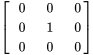
\includegraphics[scale=1, valign=c]{figures/chapter3/kernels/identity.png} & 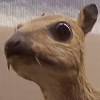
\includegraphics[scale=3, valign=c]{figures/chapter3/kernels/Vd-Orig.png}  \\
\hline
Gaussian Blur & 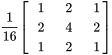
\includegraphics[scale=1, valign=c]{figures/chapter3/kernels/gaussian.png} & 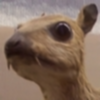
\includegraphics[scale=3, valign=c]{figures/chapter3/kernels/Vd-Blur1.png}  \\
\hline
Ridge detection & 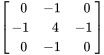
\includegraphics[scale=1, valign=c]{figures/chapter3/kernels/ridge.png} & 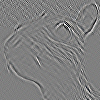
\includegraphics[scale=1, valign=c]{figures/chapter3/kernels/Vd-Rige1.png}  \\
\hline
Sharpen & 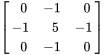
\includegraphics[scale=1, valign=c]{figures/chapter3/kernels/sharpen.png} & 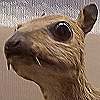
\includegraphics[scale=3, valign=c]{figures/chapter3/kernels/Vd-Sharp.png}  \\
\hline
\end{tabular}
\caption[convo]{Examplary convolutional kernels applied on an image\footnotemark. }
  \label{tab:classical_kernel}
\end{center}
\end{table}

\footnotetext{Source \url{https://en.wikipedia.org/wiki/Kernel_(image_processing)}}

% https://en.wikipedia.org/wiki/Kernel_(image_processing)
% https://towardsdatascience.com/gentle-dive-into-math-behind-convolutional-neural-networks-79a07dd44cf9
% https://towardsdatascience.com/a-comprehensive-guide-to-convolutional-neural-networks-the-eli5-way-3bd2b1164a53


\subsubsection{Convolutional layer}

A convolutional layer in a neural network is simply a layer that applies a convolutional filter. The properties of the filter, i.e. values of its elements, are learnable parameters.
Usually, in the case of colour images, there are three layers of such filters, which outputs are summed as shown in Fig. \ref{fig:conv_layer}.
The values of the filters are trained by the backpropagation algorithm.

\begin{figure}
  \centering
  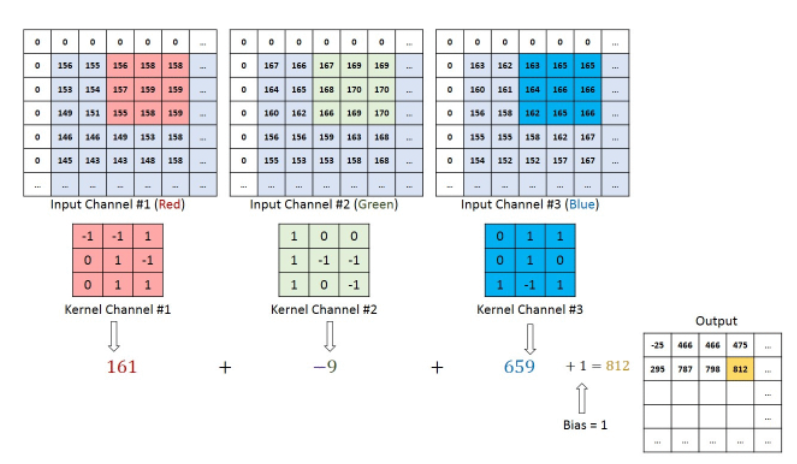
\includegraphics[width=0.9\linewidth]{figures/chapter3/convo_steps.png}
  \caption{Step of application of a convolutional filter in a neural network \protect\footnotemark}
  \label{fig:conv_layer}
\footnotetext{Source: \url{https://towardsdatascience.com/a-comprehensive-guide-to-convolutional-neural-networks-the-eli5-way-3bd2b1164a53}}
\end{figure}


The application of the convolutional filters inside the neural network creates a map of more complex filters, which can extract the spacial features and build on other convolutional layers to learn the most valuable and significant features in a given task.

\subsubsection{Pooling layers}

The pooling layers in convolutional neural networks are used to decrease the number of features and filter the most significant spatial features (equivalent of denoising). The pooling layers use windowing on an incoming input to extract values given specific criteria.
One of the popular pooling methods is max pooling.
This method outputs the biggest value in a given window (see Fig. \ref{fig:pooling_layer}).
The pooling layers do not have trainable parameters.

\begin{figure}
  \centering
  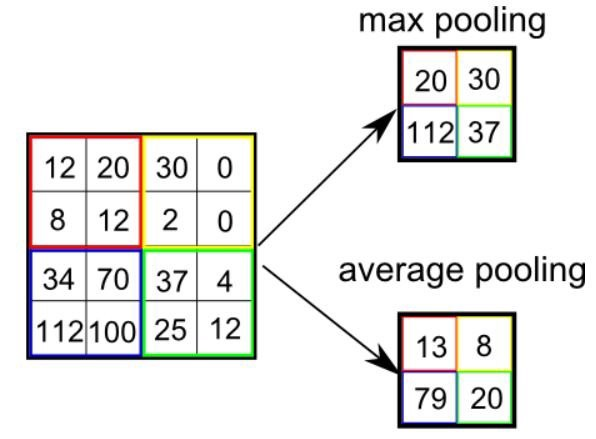
\includegraphics[width=0.6\linewidth]{figures/chapter3/avg_max_pooling.png}
  \caption{Example of max pooling and average pooling\protect\footnotemark. }
  \label{fig:pooling_layer}
\end{figure}
\footnotetext{Source: \url{https://towardsdatascience.com/a-comprehensive-guide-to-convolutional-neural-networks-the-eli5-way-3bd2b1164a53}}
\subsubsection{Convolutional networks: example architecture}

The convolutional neural networks are nowadays a standard go-to solution for solving computer vision problems.
There are many different architectures for convolutional neural networks.
This section presents an exemplary implementation of the convolutional neural network.
This architecture is known as VGG-16 \cite{https://doi.org/10.48550/arxiv.1409.1556}.

A detailed description of the network is presented in Fig \ref{fig:vgg16}.
% The detailed description of the network is presented in Table \ref{tab:vgg16} and it is visualised in Fig \ref{fig:vgg16}.

The network is considered to be a classical convolutional design.
It assumes an input of the constant size and is divided into repeated blocks of 2 or 3 convolution layers, each followed by a ReLU activation function, with the last layer in a block being a Max Pooling operation.
ReLU (Rectifier Linear Unit) function is defined as $f(x) = max(0,x)$.
This means that its value is always zero for a negative number, and in other cases, it's $x$.
Such blocks were repeated five times, with decreasing sizes in the first two dimensions and increasing in the last dimension.
The last dimension represents a convolution feature output.
After those convolutional blocks, there are three fully connected layers.
The output is a vector of size 1000, as the network was initially created for the task of categorisation on the ILSVRC data-set containing 1000 categories.

The intuition behind this architecture is that the blocks of convolutions are responsible for extracting features.
These convolutions build on top of each other and allow for more and more complex features to be learned.
The fully connected layers allow for a linear combination of these features.
Finally, the softmax function is used because it limits the output to range from 0 to 1 - which can be interpreted as a probability of given input belonging to a particular class.

% \begin{table}[h]
% \begin{center}
% \begin{tabular}{ |c|c|c|}
% \hline
% \textbf{Layer} & \textbf{Output Size} & \textbf{Parameters}\\
% \hline
% Input & 244x244x3 & \\
% \hline
% Convolution & 244x244x64 & 64 filters, 3x3 kernel\\
% \hline
% ReLU & 244x244x64 & \\
% \hline
% Convolution & 244x244x64 & 64 filters, 3x3 kernel size\\
% \hline
% ReLU & 244x244x64 & \\
% \hline
% Max Pooling & 112x112x64 &  2x2 window, 2x2 step \\
% \hline


% Convolution & 112x112x128 & 128 filters, 3x3 kernel\\
% \hline
% ReLU & 112x112x128 & \\
% \hline
% Convolution & 112x112x128 & 128 filters, 3x3 kernel size\\
% \hline
% ReLU & 112x112x128 & \\
% \hline
% Max Pooling & 56x56x128 &  2x2 window, 2x2 step \\
% \hline

% Convolution & 56x56x256 & 256 filters, 3x3 kernel\\
% \hline
% ReLU & 56x56x64 & \\
% \hline
% Convolution & 56x56x256 & 256 filters, 3x3 kernel size\\
% \hline
% ReLU & 56x56x64 & \\
% \hline
% Max Pooling & 28x28x256 &  2x2 window, 2x2 step \\
% \hline


% Convolution & 28x28x512 & 512 filters, 3x3 kernel\\
% \hline
% ReLU & 28x28x64 & \\
% \hline
% CConvolution & 28x28x512 & 512 filters, 3x3 kernel\\
% \hline
% ReLU & 28x28x64 & \\
% \hline
% Convolution & 28x28x512 & 512 filters, 3x3 kernel size\\
% \hline
% ReLU & 28x28x64 & \\
% \hline
% Max Pooling & 14x14x512 &  2x2 window, 2x2 step \\
% \hline


% Convolution & 14x14x512 & 512 filters, 3x3 kernel\\
% \hline
% ReLU & 14x14x64 & \\
% \hline
% Convolution & 14x14x512 & 512 filters, 3x3 kernel\\
% \hline
% ReLU & 14x14x64 & \\
% \hline
% Convolution & 14x14x512 & 512 filters, 3x3 kernel size\\
% \hline
% ReLU & 14x14x64 & \\
% \hline
% Max Pooling & 7x7x512 &  2x2 window, 2x2 step \\
% \hline

% Fully Connected & 4096x1 & \\
% \hline
% ReLU & 4096x1 & \\
% \hline

% Fully Connected & 4096x1 & \\
% \hline
% ReLU & 4096x1 & \\
% \hline

% Fully Connected & 1000x1 & \\
% \hline
% SoftMax & 1000x1 & \\
% \hline
% \hline
% \end{tabular}
% % https://app.neptune.ai/mmajewsk/lartpc-conv/e/LAR1-9/all?path=parameters
% \caption{\label{tab:vgg16} Detailed layers of the VGG16 architecture.}
% \end{center}
% \end{table}

\begin{figure}
  \centering
  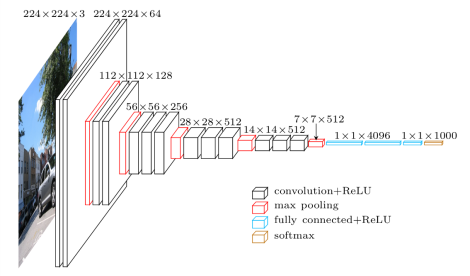
\includegraphics[width=0.9\linewidth]{figures/chapter3/vgg16.png}
  \caption{Graphical representation of the VGG16 architecture.}
  \label{fig:vgg16}
\end{figure}

% https://medium.com/mlearning-ai/an-overview-of-vgg16-and-nin-models-96e4bf398484
\section{Dimensionality reduction - Autoencoders}

High dimensionality of data sets pose a major problem for many analysis tasks.
It is often difficult to gain meaningful insights using only exploratory analysis of the data set or from simple metrics.
Additionally, sparse, high dimensional data might pose a computational problem.
Dimensionality reduction is a technique that reduces the number of dimensions of the data while retaining meaningful properties.
There are many techniques, but here I will present the most basic one that stems from neural networks.
This technique is known as autoencoder.
Autoencoder is a deep neural network whose layers can be separated into two parts, Encoder and Decoder (Fig \ref{fig:autoenc}).
The dimensionality reduction with autoencoders can be understood in the following way:
\begin{align*}
\tilde{X} = g(f(X))  \text{ where } \quad X\prime = f(X),\ g = f^{-1}
\end{align*}

The $f$ is an encoder, that reduces the input vector $X \in R^{n}$ to $X' \in R^{m}$.
The $g$ is a decoder that maps the vector $X'$ to $\tilde{X} \in R^{n}$, thus recreating the dimensionality of the initial input.
The goal of successfully trained autoencoder (encoder + decoder) is then to minimise a reconstruction error $f,g = \arg\min_{f,g} E(X-g(f(X)))$.
The above can be implemented using neural network layers and arbitrarily small $R^{m}$, which will be the intermediate output from the encoder.

\begin{figure}
  \centering
  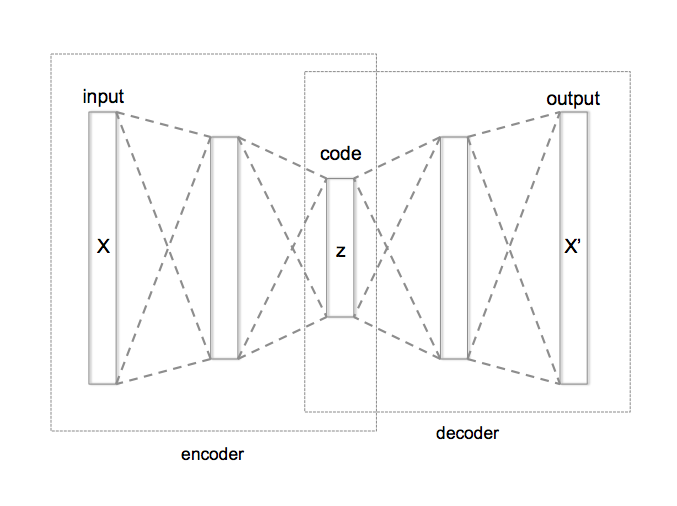
\includegraphics[width=0.5\linewidth]{figures/chapter3/Autoencoder_structure.png}
  \caption[autoenc]{Graphical representation of the autoencoder structure\footnotemark. }
  \label{fig:autoenc}
\end{figure}

\footnotetext{Source \url{https://en.wikipedia.org/wiki/File:Autoencoder_structure.png}}

The encoder part of the autoencoder network is composed of fully connected layers with diminishing size, up to the desired size of the dimension required by the reduction.
The last layer of the encoder is connected to the decoder part of the network, comprising fully connected layers growing in size up to the original input size.

The encoder tries to compress the information to a smaller dimension (also called the latent space), while the encoder tries to uncompress this information and recreate objects from the original data space of dimensionality $n$.


\section{Recurrent networks}

Modelling of the ordered data sets is a very popular task and employs a special type of deep artificial neural networks. For instance we would like to preserve a temporal information for the modelled series of data points, where the next element may be influenced by the previous ones.
Such a goal can be achieved by using recurrent connections in neural networks.
The recurrent connection can be understood as a loop in a neural network graph.

%  https://en.wikipedia.org/wiki/Recurrent_neural_network
\subsection{Standard recurrent network}
% https://stanford.edu/~shervine/teaching/cs-230/cheatsheet-recurrent-neural-networks
% https://colah.github.io/posts/2015-08-Understanding-LSTMs/

Generally we can describe the output from a simple recurrent neural network as follows:
\begin{equation}
h_t = \sigma_h(W_{h} x_t + U_{h} h_{t-1} + b_h)
\end{equation}
\begin{equation}
y_t = \sigma_y(W_{y} h_t + b_y)
\end{equation}

Where elements $W_{h}, U_{h}, W_{y}, b_{h}, b_{y}$ are weights shared in the temporal dimension, and assuming that $\sigma_{h},\sigma_{y}$ are activation functions.

The $h_{t}$ term is a recurrent output, which will be used in the next forward pass of the network.
It is composed of a current input $x_{t}$ and the previous looped connection output $h_{t-1}$.
That recurrent output is also used to create the output of the neural network $y_{t}$.
Neural networks can be represented as unrolled in time dimension (Fig \ref{fig:unroll_rec}).
Recurrent neural networks can be divided into categories based on the input, output and recurrent connection configuration (Fig \ref{fig:recurrent_div}).

\begin{figure}
  \centering
  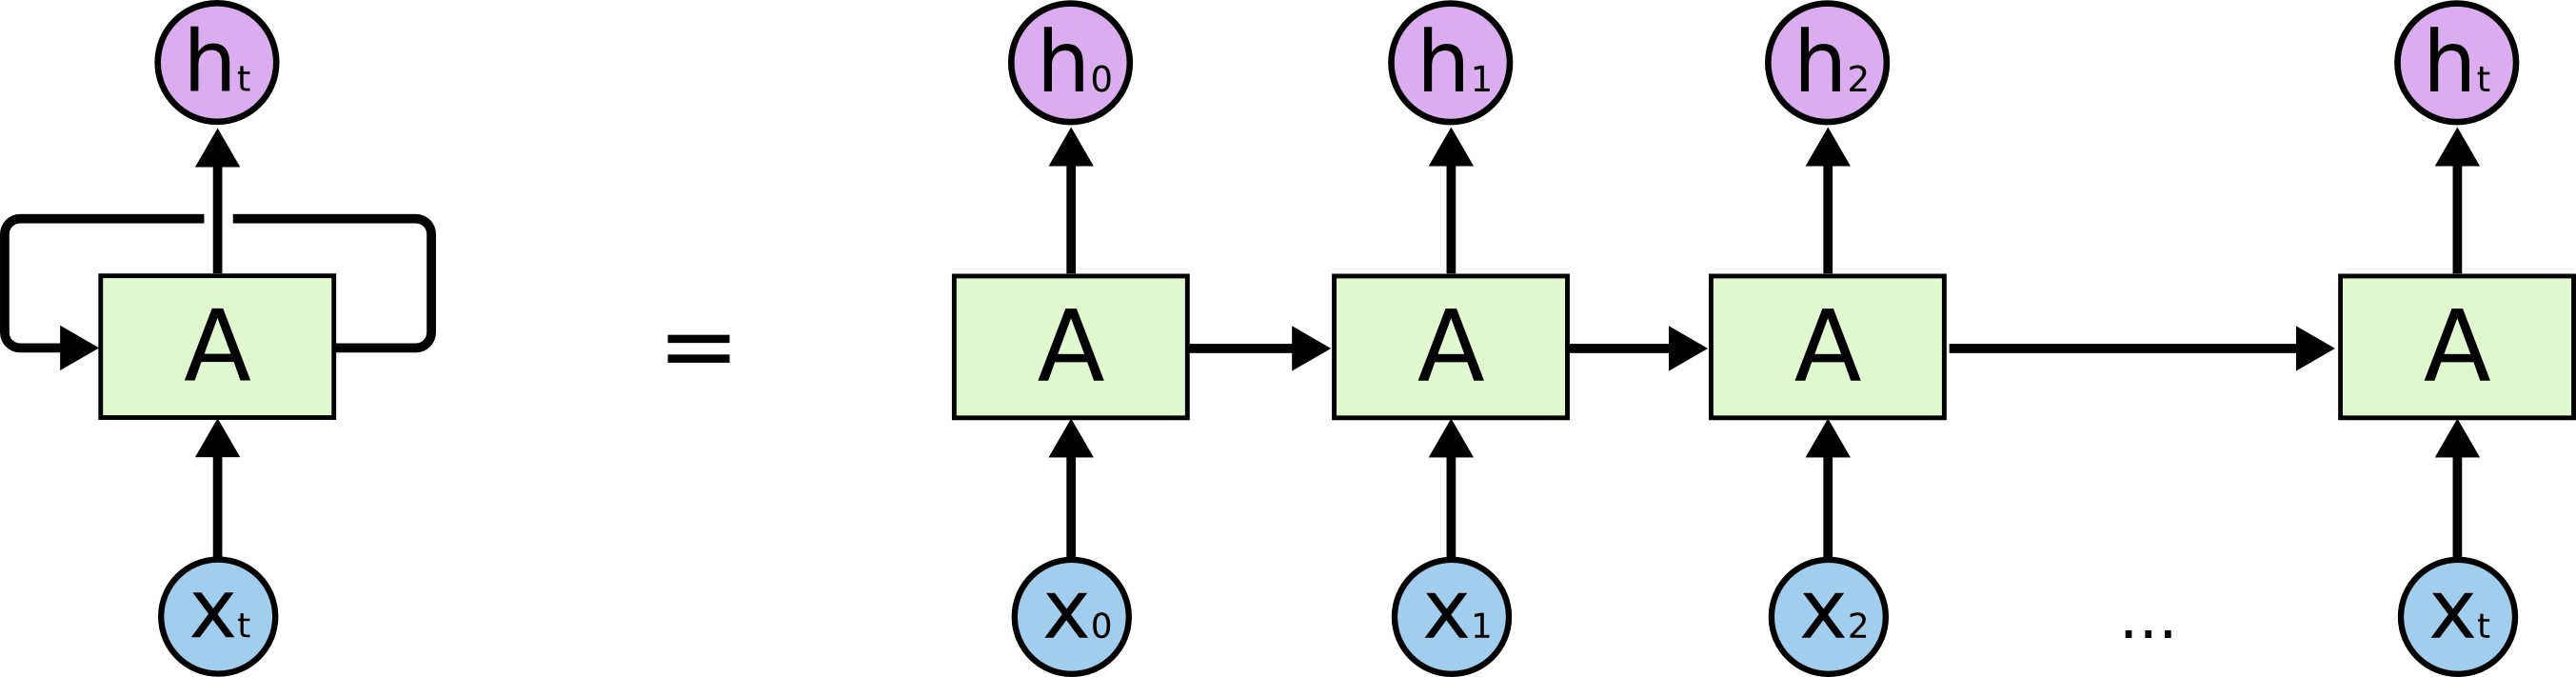
\includegraphics[width=0.9\linewidth]{figures/chapter3/RNN-unrolled.png}
  \caption{A representation of a simple neural network.
   The left representation is the rolled representation, and the right is a representation unrolled in the time dimension.}
  \label{fig:unroll_rec}
\end{figure}

\begin{figure}
  \centering
  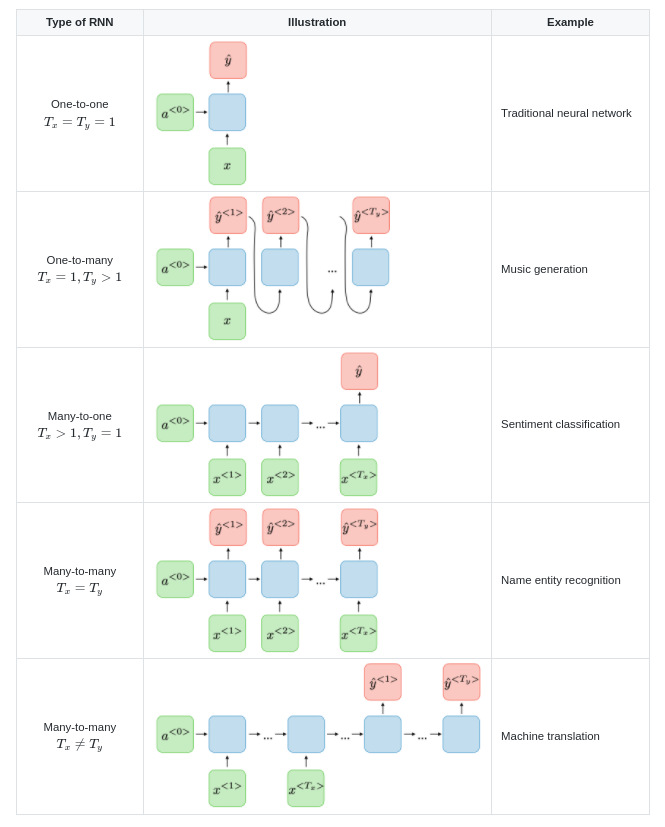
\includegraphics[width=0.9\linewidth]{figures/chapter3/rnn_placeholder.png}
  \caption[recu]{Different recurrent neural networks, unrolled in time. The first example at the top is just a regular neural network. The second row represents a neural network which uses a single output and continuously produces output as many times as desired. The third row represents an inverted example when the network accumulates several different time step inputs and has a single output. This method can be helpful in sentiment analysis when a singular output marking sentiment is desired after a sequence of words.
  The fourth example depicts a RNN, which continuously produces output for each timestep. The last row shows that the number of inputs and outputs can be changed according to particular requirements\footnotemark. }
  \label{fig:recurrent_div}

  \footnotetext{ Source: \url{https://stanford.edu/~shervine/teaching/cs-230/cheatsheet-recurrent-neural-networks}}

\end{figure}


The pitfall of the regular RNNs is their poor performance in tasks that require long term memory (tasks that require the model to hold certain information for an extended amount of time).
Also, in the backward pass in RNN's there is a problematic partial differentiation $\frac{h_{t}}{h_{t-1}}$. If this term is consistently less or greater than 1, it may, in the end, cause this gradient to diminish to values close to 0 or reach very large values. This is also called the vanishing/exploding gradient problem.

\subsection{LSTM}

The problems of the classical RNNs are partially solved by LSTM (Long short-term memory) architecture. It can retain information for more extended periods and partially solves the problem of vanishing/exploding gradient.

\begin{figure}[H]
\centering
\begin{subfigure}[b]{0.5\textwidth}
    \centering
\begin{align*}
& f_t = \sigma_g(W_{f} x_t + U_{f} h_{t-1} + b_f) \\
& i_t = \sigma_g(W_{i} x_t + U_{i} h_{t-1} + b_i) \\
& o_t = \sigma_g(W_{o} x_t + U_{o} h_{t-1} + b_o) \\
& \tilde{c}_t = \sigma_c(W_{c} x_t + U_{c} h_{t-1} + b_c) \\
& c_t = f_t \circ c_{t-1} + i_t \circ \tilde{c}_t \\
& h_t = o_t \circ \sigma_h(c_t)
\end{align*}
% \caption{Neutrino}
%     \label{plot:cross_neu}
  \end{subfigure}
\begin{subfigure}[b]{0.45\textwidth}
    \centering
    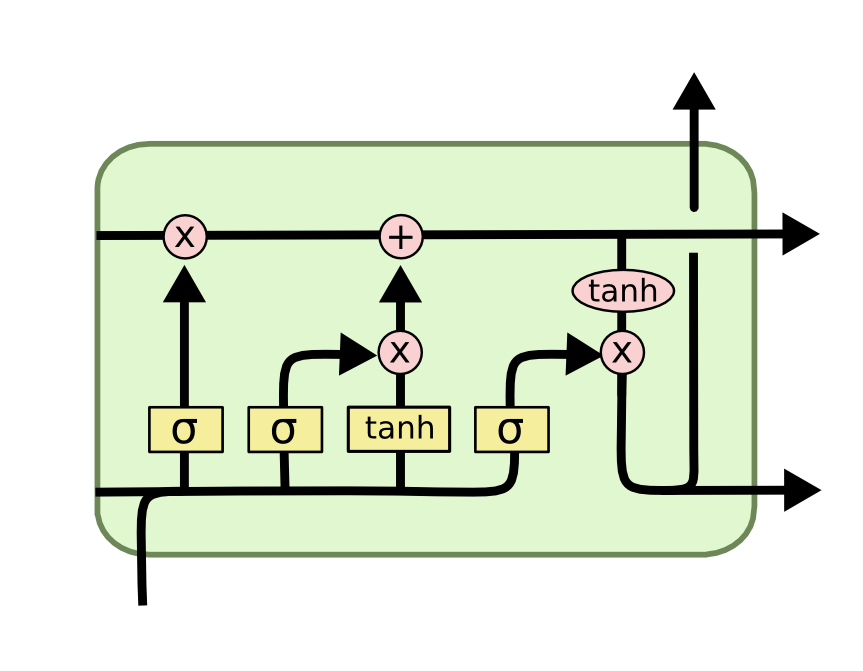
\includegraphics[width=\linewidth]{figures/chapter3/lstm.png}
  \end{subfigure}
\caption[lstm]{Architecture of LSTM. LSTM in equation form on the left and in graphical form on the right\footnotemark. }
\label{fig:lstm}
\end{figure}

\footnotetext{Source: \url{https://colah.github.io/posts/2015-08-Understanding-LSTMs/}}
%https://en.wikipedia.org/wiki/Long_short-term_memory
%https://colah.github.io/posts/2015-08-Understanding-LSTMs/

Fig. \ref{fig:lstm} presents LSTM, there $\sigma_g$ is sigmoid function, and the $\sigma_{c}$ and $\sigma_{h}$ are hyperbolic tangents.
The LSTM's inner workings can be explained intuitively. The $c_{t}$ vector can be assumed to represent the memory of the layer, as it is passed in  a time dimension. $f_{t}$ values range from 0 to 1, and thus can either let the values of $c_{t}$ continue to propagate (multiplied by 1) or forget them (multiply by 0). The $i_{t}$ values range from -1 to 1, and can add the new values to $c_{t}$.

\subsection{WTTE-RNN}
\label{sec:wtte_rnn}

\begin{figure}
  \centering
  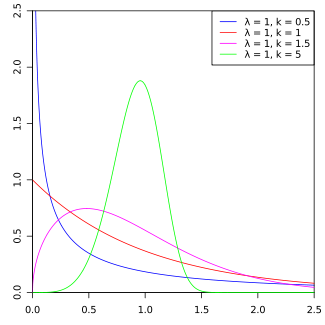
\includegraphics[width=0.5\linewidth]{figures/chapter3/325px-Weibull_PDF.svg.png}
  \caption[wei]{Weibull distribution with examplary paremeters\footnotemark. }
  \label{fig:weibull}
  \footnotetext{Source: \url{https://stanford.edu/~shervine/teaching/cs-230/cheatsheet-recurrent-neural-networks}}

\end{figure}

Another enhancement to the RNN models can be achieved by coupling them with the Weibull distribution. In that way we can create a model that can be able to predict a specific event (for instance time of the next aircraft engine checkup).
The Weibull distribution (Fig. \ref{fig:weibull}) is defined by the following equation:
\begin{equation}
f(x;\lambda,k) =
\begin{cases}
\frac{k}{\lambda}\left(\frac{x}{\lambda}\right)^{k-1}e^{-(x/\lambda)^{k}} & x\geq0 ,\\
0 & x<0,
\end{cases}
\end{equation}

The Weibull distribution is often used for modelling the ``time-to-failure'' in the survival analysis.
For assessing the probability of an event (churn/survival), a version of Weibull log-likelihood is used (proposed in WTTE-RNN \cite{martinsson:Thesis:2016}):
\begin{equation}
    \lambda(t) = (t/\alpha)^{\beta-1}\beta/\alpha
\Lambda(t) = (t/\alpha)^{\beta}
\end{equation}


Where $\lambda(t)$ and $\Lambda(t)$ are hazard function and cumulative hazard function derived from Weibull's distribution.
The term $\alpha$ and $\beta$ are scale and shape parameters. In this case the value of beta is set to be constant $\beta = 1$.
For incorporation of this distribution with the recurrent network, a log-like likelihood is used in the following form:
$$
Loss = u * log(e^{\Lambda(t+1)-\Lambda(t)}-1 - \Lambda(y+1))
$$

And the custom activation function:

\begin{equation}
    activation(x_{i}) = e^{x_{0}} + Softplus(x_{1})
    \label{math:acti}
\end{equation}

\section{Deep Reinforcement learning}

Many of the tasks in the real world do not have easy do define metrics and cannot follow input - output model of learning.
In some areas, a reward response is more straightforward to define than the exact desired output.
An example of this may be a game of chess - it is hard to define what set of moves will win with a given opponent, and in the end, there is only a win-lose response.
Such problems are solved with Reinforcement Learning \cite{Lapan18}.

\subsubsection{RL formalism's}
\label{sec:rl_mdp}

As mentioned previously, reinforcement learning focuses on the action being taken in a specific environment.
This is represented on the flowchart in Fig. \ref{fig:rl_env_flow}.
More formally, in RL there are two important entities: \textbf{Agent} and \textbf{Environment}.
The agent is an entity operating in the environment via \textbf{action}.
The environment provides agent with \textbf{observation} and \textbf{reward}.
While the observation expresses the state of the environment, the reward expresses how well the agent performed.


\begin{figure}
  \centering
  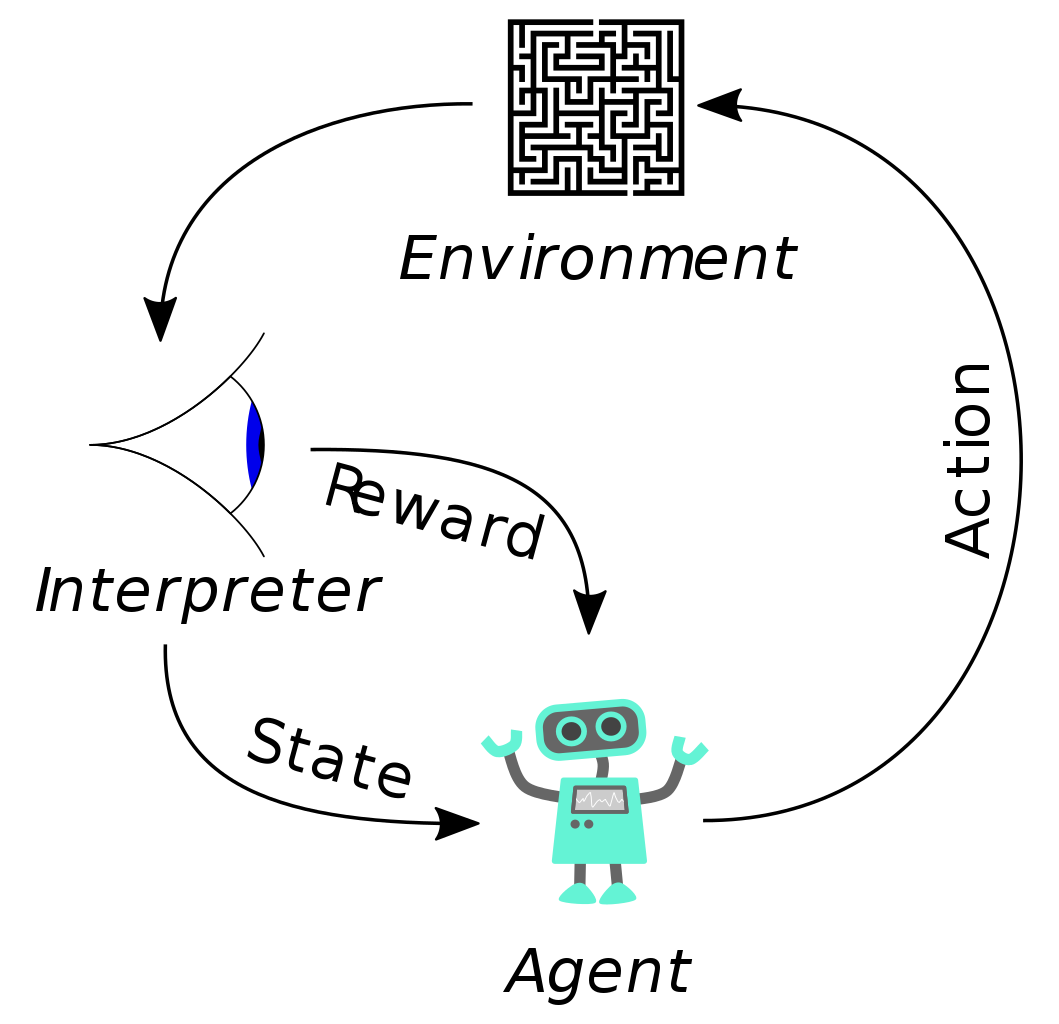
\includegraphics[width=0.4\linewidth]{figures/chapter3/Reinforcement_learning_diagram.svg.png}
  \caption[rlenv]{A diagram of the flow of information in a reinforcement learning setting\footnotemark.}
  \label{fig:rl_env_flow}
\end{figure}
\footnotetext{Source: \url{https://commons.wikimedia.org/wiki/File:Reinforcement_learning_diagram.svg}}

The environment in RL is usually expressed as an MDP (Markov decision process).
For that, the system (environment) is expressed as observable and distinguishable \textbf{states} $s$.
All of the observable states create state space $S$.
In MDP, the system states have Markov property, meaning that the following state is only dependent on the current state, not the previous states.
This assumption is not valid for many of the environments and problems that actually have been solved with reinforcement learning.
Also all of the possible \textbf{actions}  $a$ create action space $A$.
The relation of action and states is expressed as function $P_{a}=Pr(s_{t} | s_{t-1}, a_{t})$, which assigns a probability of a state given a previous state and action.
And finally, the \textbf{reward} is expressed as $R_{a}=R(s_{t}, s_{t-1}, a_{t})$, where an immediate reward is given for transition from $s_{t-1}$ to $s_{t}$ given action $a_{t}$.
Those factors are usually expressed as MDP tuple $(S, A, P_{a}, R_{a})$.
The last important element in the MDP formalism is policy $\pi$.
$\pi(a|s)$ is a probabilistic mapping from $S$ to $A$. The goal of MDP is to find a mapping $\pi$ which maximises the reward.

\subsection{Q-Learning}

As stated before, reinforcement learning is seeking to maximise the cumulative reward.
We can define this cumulative reward as return $G_{t}$, as a sum of the rewards in the ongoing time-steps \cite{Sutton1998}:
\begin{align}
  G_{t} = R_{t+1} +  \gamma R_{t+2} + \gamma^{2} R_{t+2} + \ldots =   \sum_{t=0}^{\infty} r_{t}\gamma^{t}
\end{align}
The $\gamma$ ($0 \leq \gamma \leq 1$) term in the equation above is called discount.
It is used to parameterise and asses the greediness of the algorithm by discounting future rewards.

Q-learning is an algorithm for solving reinforcement learning problems.
It is also known to belong to a subset of algorithms known as Value-based algorithms.
This means the algorithm uses a state-value function $V(s)$, as defined in \ref{eq:value}

\begin{align}
  V(s) = \mathbb{E} \left[  G_{t} \bigg| s_{t} \right]
  \label{eq:value}
\end{align}

In plain words: value is the sum of all possible future discounted ($\gamma$) rewards ($r$).
The value can also be applied to an action, as after applying an action, the new state and its reward are given.
Assuming a policy $\pi$, we can also define a value of state s under the policy:

\begin{align}
  V_{\pi}(s) = \mathbb{E}_{\pi} \left[  G_{t} \bigg| s_{t} \right]=\mathbb{E}_{\pi} \left[  \sum_{t=0}^{\infty} r_{t}\gamma^{t} | s_{t} \right]
  \label{eq:valuepolicy}
\end{align}

We can also define a q-function $Q_{\pi}$, which given a state and action identifies the value.
\begin{align}
  Q_{\pi}(s,a) = \mathbb{E}_{\pi} \left[  G_{t} \bigg| s_{t}, a_{t} \right]
  \end{align}

We can extend Eq. \ref{eq:valuepolicy} to the recurrent form, as the value function is dependant on future value functions.
\begin{align}
V_{\pi}(s) = \sum_{a}\pi(a|s)\sum_{s',r}p(s',r|s,a)\left[r+ \gamma v_{\pi}(s')\right]
\label{eq:belman1}
\end{align}

Eq. \ref{eq:belman1} is called Bellman equation and represents the connection between the current value and future value.

For both state-value and action-value functions we can define optimal functions:

\begin{align}
v_{*}(s) = \max_{\pi}v_{\pi}(s)
q_{*}(s,a) = \max_{\pi}a_{\pi}(s,a)
\label{eq:belman2}
\end{align}

Those are the optimal functions in sense of using the policy that maximises the value.

The belman optimiality equations for $q_{*}(s,a)$ is:
\begin{align}
q_{*}(s,a) = \sum_{s',r}p(s',r|s,a)\left[r+ \gamma max_{a'}q_{s}(s',a')\right]
\label{eq:belman3}
\end{align}

The optimal q action-value function may be aproximated by using a action-value table $Q(S_{t}, A_{t})$.
This table can be iteratively filled by choosing the actions using the policy derived by Q.

\begin{align}
% & Q(S,A) \leftarrow Q(S,A) + \alpha\left[R+ \gamma max_{a}Q(S',a) - Q(S,A)\right] \\
& Q(s,a) \leftarrow r + \gamma \max_{a'} Q(s',a') \\
& Q(s,a) \leftarrow (1-\alpha)(Q(s,a)) + \alpha(r + \gamma \max_{a'} Q(s',a'))
\label{eq:Qlearning}
\end{align}

The last equation above is the key equation begin the q-learning algorithm.
This table can approximate the optimal solution to the given reinforcement learning problem.
You can notice that the $Q$ should contain all of the different state-action pairs, which for many problems is not practical.
This is where the Q-learning turns to the neural network's algorithms, as instead of using the $Q$ table, we can approximate $Q$ using a neural network.


%https://web.stanford.edu/class/psych209/Readings/SuttonBartoIPRLBook2ndEd.pdf
% https://www.mlq.ai/reinforcement-learning-policies-value-functions-bellman-equation/
% https://www.analyticsvidhya.com/blog/2021/02/understanding-the-bellman-optimality-equation-in-reinforcement-learning/
% https://towardsdatascience.com/reinforcement-learning-markov-decision-process-part-2-96837c936ec3
\subsection{Deep Q-Learning}
\label{sec:dqn}

Given that there exists an optimal bellman action-value function $Q^{*}(s',a')$ \cite{https://doi.org/10.48550/arxiv.1312.5602} and it's value in the next time-step given the state $s'$ and action $a'$ is known, then the optimal strategy is to select an action which maximises the expected value of future reward:

\begin{align}
  Q^{*}(s,a) = E_{s' \sim \epsilon} \left[ r + \gamma \max_{a'} Q^{*}(s',a') \bigg| s,a \right]
\label{eq:deepQlearning}
\end{align}

In terms of a target for the neural network, this can be specified as:

\begin{align}
 Y_{t}^{Q} =  R_{r+1} + \gamma \max_{a} Q(S_{t+1},a; \theta_{t})
\label{eq:deepQlearningTarget}
\end{align}

The basic idea of Q-learning is to update the Q function/table iteratively with the above equation.
As stated previously, this may not be practical and lacks generalisation.
Instead, a parameterised function an approximate one may be used $Q(s,a;\theta) \approx Q^{*}(s,a)$.
This $Q$ function approximator can be a neural network parameterised by weights $\theta$.
Next, we can build a loss function $L_{i}(\theta_{i})$
\begin{align}
L_{i}(\theta_{i}) = \mathbb{E}_{s,a~p(\dot)}\left[(y_{i} - Q(s,a;\theta))\right]
\end{align}

where $y_{i} = \mathbb{E}_{s'~\epsilon}\left[r+\gamma \max_{a'}Q(s',a';\theta_{i-1})\right]$

Assuming MSE as our loss metric, we can write down loss function as follows:
\begin{align}
\mathcal{L} = (Q(s,a,\theta) - (r+\gamma\max_{a'}Q(s',a';\theta_{i-1d})))^{2}
\end{align}

This, in practice, creates a particular problem, as we need to process the states and the actions in the neural network Q twice, once to get the output that will be compared with the prediction and once to calculate future prediction. This creates a loop that can lead to the network's instability, as it will be chasing a target that is constantly changing. This is why usually, in practice, there are two separate networks (target network), one for calculating the prediction and the other for calculating the output.

\subsection{Experience replay buffer}

In the simple approach to reinforcement learning using DQN, the model would be trained on the rewards, states and actions that have been just exchanged with the environment.
This means that there would have to be a step in the environment for each training sample.
Additionally, this would make the model training less stable, as the recently visited states would directly impact the model the most.
Because of this, for the model training, an experience replay buffer is used.
The replay buffer (or memory buffer), is used to store the MDP tuples received from the environment instead of using them immediately and discarding them.
The training and the exploration are logically separated.
After a period of exploration (interaction with the environment), the training process begins on the gathered samples.
There are multiple ways to implement a replay buffer, but one of the most common one is to create a limited length list (first in - last out), where the old samples are discarded.
Then such a list is randomly sampled for the training cases.

\subsection{Deep Double Q-Learning}

One of the problems of the DQN algorithms is over-optimistic value estimates.
This is because when selecting the maximal value in the $\max_{a} Q(S_{t+1},a; \theta_{t})$ term we use one network pass to both choose (selecting the action of the max value), and calculating it's value (by returning only the maximum).
The deep double q-learning algorithm \cite{https://doi.org/10.48550/arxiv.1509.06461} aspires to solve this problem by using an additional step of the network (eq. \ref{eq:doubleQlearning}).

\begin{align}
 Y_{t}^{DoubleQ} =  R_{r+1} + \gamma Q(S_{t+1}, \max_{a} Q(S_{t+1},a; \theta_{t}); \theta'_{t})
\label{eq:doubleQlearning}
\end{align}

This calculation of the target $Y$ is done using two sets of networks. Network $\theta_{t}$ is the network that is currently online learning and is used to pick the action, but the network $\theta'_{t}$ is used to estimate the value of this action.
The values of $\theta'_{t}$ can be updated periodically with the weights of $\theta_{t}$.
This can also be done using blending of the parameters $\theta'_{t+1} = \beta \theta'_{t} + (1-\beta)\theta_{t}$ wehere $0<\beta<1$.

\section{Probabilistic programming}
%https://nbviewer.org/github/CamDavidsonPilon/Probabilistic-Programming-and-Bayesian-Methods-for-Hackers/blob/master/Chapter1_Introduction/Ch1_Introduction_PyMC3.ipynb
%https://pymcmc.readthedocs.io/en/latest/theory.html
%https://docs.pymc.io/projects/examples/en/latest/samplers/SMC2_gaussians.html
% https://nbviewer.org/github/CamDavidsonPilon/Probabilistic-Programming-and-Bayesian-Methods-for-Hackers/blob/master/Chapter3_MCMC/Ch3_IntroMCMC_PyMC3.ipynb
%
%https://towardsdatascience.com/from-scratch-bayesian-inference-markov-chain-monte-carlo-and-metropolis-hastings-in-python-ef21a29e25a
%
%https://arxiv.org/pdf/1504.01896.pdf

Probabilistic programming \cite{davidsonpilon2015probabilistic} was born out of the Monte Carlo simulations and Bayesian reasoning. In brief: it uses a probabilistic approach to modelling and machine learning.
It is considered to be a white-box approach.
Probabilistic programming uses Markov Chain Monte Carlo (MCMC) to sample probability distribution function.


\subsection{Metropolis-Hastings algorithm example}

Metropolis-Hastings algorithm  \cite{Robert2004} is an MCMC based algorithm used for sampling a probability distribution.
This process can also be used to approximate the distribution.
Let's assume function $f(d_{i})$ that is a probability density function:

\begin{align}
f(d_{i}) = \frac{1}{\sigma \sqrt{2\pi} } e^{-\frac{1}{2}\left(\frac{d_{i}-\mu}{\sigma}\right)^2}
  \end{align}

This function is parametrised by two parameters.
Let's assume that the $\mu = 0$ is already known, and let's describe the unknown parameter $\theta = \sigma$.
The task at hand is to approximate the $f(d_i)$.
Now, at it's core, all Bayesian methods use simple, yet powerful Bayes theorem:

\begin{align}
  P(\theta|D) = \frac{P(D|\theta)P(\theta)}{P(D)}
\end{align}

$P(\theta|D)$ is called posterior, $P(D|\theta)$ is the likelihood, $P(\theta)$ is the prior, and $P(D)$ is the evidence.
In the case of machine learning tasks, we have data to test our beliefs, and so in this case, in order to find the approximation of $f(d_{i})$, we would like to find the probability distribution of $\theta$ under the condition of existing data $D$.

For this purpose we can say that the following approximation is true:
\begin{align}
f(x_{i} | \theta) \approx P(D|\theta)
  \end{align}

The Metropolis-Hastings method uses a transition model $Q(\theta'|\theta)$ to generate candidates for the searched parameter $\theta$.
In this algorithm, $Q$ is used for creating random steps $\theta$ in the distribution space.
For example $Q$ can be defined as $Q(\theta'|\theta)=N(\theta, \mu)$ and that $\mu=1$ - a random walk.
With each step, we assess if the new position $\theta'$ is more likely to fit the distribution.
If it is not, we discard the newly generated position and sample again.
Each step is directly influenced only by the previous step, which means it satisfies the Markov chain rule.
The test of the likelihood of the step more likely belonging to distribution can be described as a ratio:

\begin{align}
  R = \frac{P(\theta'|D)}{P(\theta|D)}
\end{align}

Which can be expanded with the Bayes theorem, and then expressed in terms of a PDF

\begin{align}
  R = \frac{P(D|\theta')P(\theta')}{P(D|\theta)P(\theta)} =\frac{ \prod_{i}^{n}f(d_{i}|\theta')P(\theta') }{\prod_{i}^{n}f(d_{i}|\theta)P(\theta)}
\end{align}

Then the acceptance probability can be explained as:

\begin{align}
    A(R)=
\begin{cases}
    R, & \text{if } R < 1 \\
    1,& \text{otherwise}
\end{cases}
      \label{eq:acceptance}
\end{align}

The eq. \ref{eq:acceptance} means that we will accept new $\theta^{\prime}$ if the ratio $R$ is greater than $1$, but otherwise, we will accept it with probability $R$.

The steps of the Metropolis-Hastings algorithm can be described as the pseudo-code in Listing \ref{alg:metropolis}.
The first step is to generate random $\theta$. Then, we generate $\theta\prime$, and calculate the probability of belonging to the distribution for $\theta$ and $\theta\prime$. Then we use the acceptance rule to either accept or reject $\theta\prime$ as new $\theta$. Those steps are repeated $k$ times.


\begin{algorithm}[ht]
  \caption{Steps of Metropolis-Hastings algorithm }
  \label{alg:metropolis}
\KwData{$\theta \gets random$}
\For{$k \in \{1,\dots,K\}$}{

  $\theta\prime \gets Q(\theta$)

  $prob\_theta \gets f(\theta)$

  $prob\_theta\prime \gets f(\theta\prime)$

  $R \gets \frac{prob\_theta\prime}{prob\_{theta}}$

  \uIf{uniform\_random(0,1) $> R $ }{

    $\theta \gets \theta\prime$
  }
}
\end{algorithm}


The process described in the listing \ref{alg:metropolis} creates a ``trace'' of candidate $\theta$ parameters, as visualised in Figure \ref{fig:random_walk}.

\begin{figure}
  \centering
  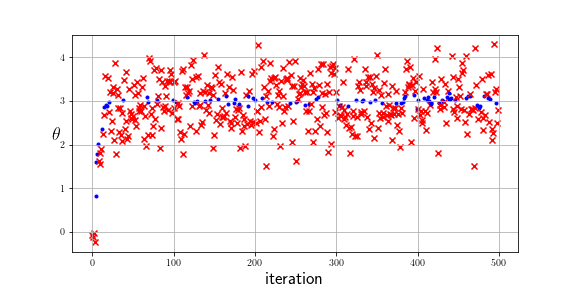
\includegraphics[width=0.9\linewidth]{figures/chapter3/random_walk.png}
  \caption{ Exemplary steps of Metropolis-Hastings steps. In this example, the target distribution is $\mathcal{N}(\mu=0, \sigma=3)$. The accepted values are in blue, and the red crosses are rejects.}
  % source: assets/random_walk
  \label{fig:random_walk}
\end{figure}


\subsubsection{Tuning in Metropolis}
\label{chap3:tuning_metropolis}

The simple version of the Metropolis-Hastings algorithm assumes that the proposed $\theta\prime$ comes from a random walk $Q(\theta'|\theta)=N(\theta, \mu)$ with $\mu=1$ but this creates a problem.
Depending on the type of the task, the variance $\mu$ of the sampled distribution can result in either too small or too big steps.
An additional effort can be made to find a step size $\mu$ better suited for our particular case.
It has been proven that one of the good indicators of a well-picked step $\mu$ is the acceptance rate of $23.4\%$ \cite{10.1214/aoap/1034625254}.
We set a tuning parameter as several additional steps of the algorithm that will be used to find a proper $\mu$ for the rest of the run \cite{colin_carroll_2019}.

\subsection{Probabilistic programming and Bayesian modelling}

Probabilistic programming is a combination of programming paradigm and probabilistic modelling.
It is usually conducted using programming frameworks, such as PYMC3 \cite{Salvatier2016}, and allows for automatic inference of the models.

Depending on the use case, it bears the marks of machine learning, as it is possible to obtain models via training (approximation of the parameters).
The critical difference with ML methods such as neural networks is that in the probabilistic modelling, the models have to be defined at least approximately.
This means that some knowledge of the statistical nature of the underlying modelled processes is necessary.

It also means that the trained model is not a black box, and its analysis can provide helpful insight and understanding of the model.
Another advantage of Bayesian modelling is its generative capabilities.
The MCMC process can be used to obtain the needed parameters (usually by taking the expectation value of the generated distribution).
Then, these parameters can be used in the assumed underlying properties and distributions to generate synthetic samples of the data.

\section{Clustering}
\label{sec:clustering}

In the general case, clustering is a process of grouping unlabeled data points into clusters that segregate cases with similar traits. There are many different clustering algorithms, each with its own preferred use case. In this section, I will present the most basic algorithm known as the K-means and two algorithms used in the later chapters. All of the presented algorithms are implemented as a part of the scikit-learn \cite{scikit-learn} package.

\subsection{K-means}

K-means (Fig. \ref{fig:kmeans}) clustering is a very basic algorithm. It divides the dataset absolutely (all of the points belong to a cluster) and expects the number of clusters $k$ as the input.

The algorithm can be initialised by picking $k$ data points randomly, and treating them as initial clusters' centroids $m_{k}$.
Then, for the remaining data points the distance to each of the centroids is calculated $|x_{i} - m_{k}|$.
Data points are assigned to the nearest centroids, and the set of the points assigned to each centroid creates a cluster.
The last step of the algorithm is to recalculate the centroids $m^{(t+1)}_k = \frac{1}{\left|S^{(t)}_k\right|} \sum_{x_j \in S^{(t)}_i} x_j $

% https://scikit-learn.org/stable/modules/clustering.html#k-means

\begin{figure}
  \centering
  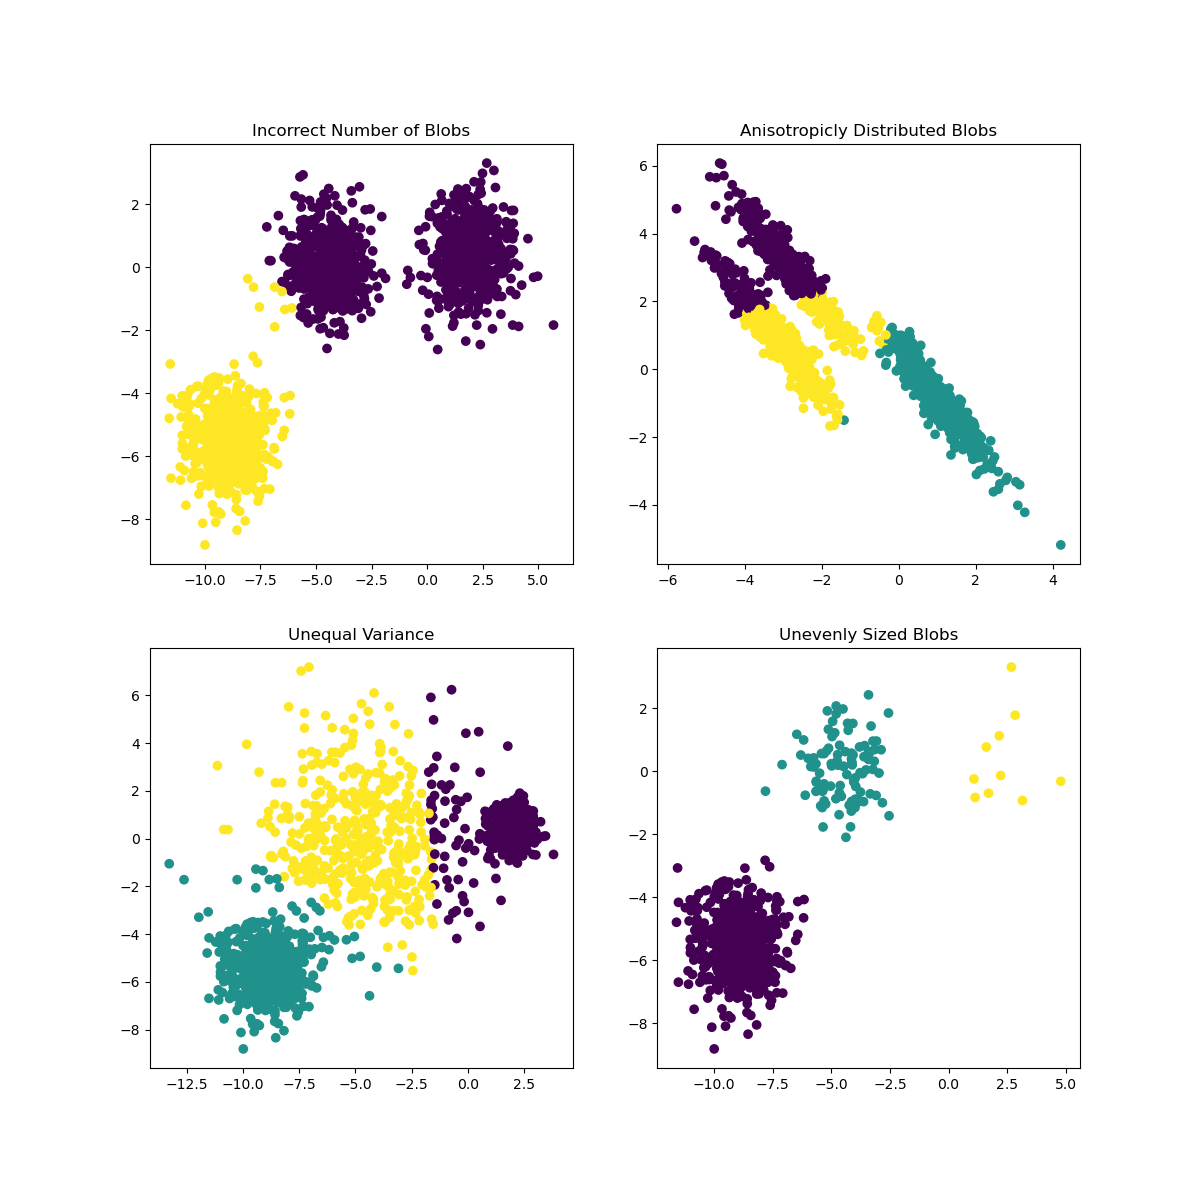
\includegraphics[width=0.6\linewidth]{figures/chapter3/sphx_glr_plot_kmeans_assumptions_001.png}
  \caption{Performance of the k-means algorithm on synthetic datasets. The upper left plot shows the effect of the algorithm using k=2, but the data clearly has 3 clusters. The right upper plot shows how the k-means fails to work with anisotropically distributed data, and the lower-left plot shows how it performs with the data of unequal variance. The last lower right plot shows an ideal case of a k-means algorithm with a proper number of clusters, with equal variance and isotropically distributed data. }
  % source: assets/random_walk
  \label{fig:kmeans}
\end{figure}


\subsection{DBSCAN}

In contrast to the K-means clustering, the DBSCAN\cite{Ester96adensity-based} (Fig. \ref{fig:dbscan}) algorithm does not divide the dataset absolutely, as it doesn't assign all data points to clusters (there are points that do not belong to any cluster - outliers). Additionally, it does not require a number of clusters as the input.
It does require a minimum number of points $MinPts$ and a minimum distance $\epsilon$.

The most important for understanding how the DBSCAN algorithm works is the idea of  ``core points''.
A point $p$ is considered to be the core point if in the range lower than $\epsilon$ there is at least $MinPts$.

The steps of the algorithm can be described as follows:

\begin{figure}
  \centering
  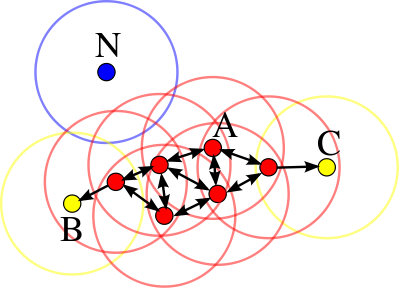
\includegraphics[width=0.45\linewidth]{figures/chapter3/400px-DBSCAN-Illustration.svg.png}
  \caption[dbscan]{A representation of the DBSCAN clustering. The blue N dot is a noise point, as it does not contain any point within the given $\epsilon$. The red points have at least two other neighbours and thus are core points. The yellow B and C points are border points as they are only connected by one other point.\footnotemark }
  \label{fig:dbscan}
\end{figure}

\footnotetext{Source: \url{ https://commons.wikimedia.org/wiki/File:DBSCAN-Illustration.svg}}



\begin{center}
\begin{enumerate}
\item The algorithm starts by choosing an arbitrary point $p$ in the dataset.
\item First, the neighbouring points $q$ that satisfy $ distance(p,q) < \epsilon$ are pushed onto the stack for further processing.
\item If the number of $q$ is equal or greater than $MinPts$, then the point $p$ is considered to be a ``core point'', and is assigned to the current cluster.
\item If that number is lower than $MinPts$, but one of those points is the core point, then $p$ is the border point and also is assigned to the current cluster.
\item If none of the above applies, then $p$ is labelled as ``noise''.
\item The process repeats by popping the stack and getting new $p$.
\end{enumerate}
\end{center}

The DBSCAN algorithm can be understood as density clustering.
If for two points $p$ and $q$ the following is true: $p$ is a core point, and $q$ is a core point, and  $distance(p,q) < \epsilon$, then we say that those points are joined by density edge.
If for any two points $p$ and $q$ in the graph created by density edges there exists a path, then $p$ and $q$ are density connected.
In this sense, we can say that any two points in a cluster are density connected.

\subsection{OPTICS}
% https://scikit-learn.org/stable/modules/clustering.html#optics
% https://towardsdatascience.com/clustering-using-optics-cac1d10ed7a7
% https://livebook.manning.com/book/machine-learning-for-mortals-mere-and-otherwise/chapter-18/65
% https://towardsdatascience.com/understanding-optics-and-implementation-with-python-143572abdfb6

The OPTICS \cite{10.1145/304182.304187, rhys2020machine} algorithm can be thought of as an extension of the DBSCAN, although by itself, it only provides a way of ordering points without assigning them to clusters.
OPTICS requires only the minimum number of neighbouring points with respect to a core point $MinPts$, and the maximum allowed distance for a core point $\epsilon_{max}$ is optional but can speed up calculations.
It introduces two important notions:

\begin{description}
   \item[Core-distance] - the minimum value of $\epsilon$ that makes the point a core point, given $MinPts$. The $core\_distance$ can be as small as needed but no bigger than $\epsilon_{max}$.
   \item[Reachability-distance] - a measure between two points $p$ and $q$. It can be expressed as \\ $max(core\_distance(q), distance(p,q))$ if q is a core point. It is undefined if $q$ is not a core point.
  \item[Reachability-score] - calculated per point. If $p$ is a core point then this value is equal to $core\_distance$ otherwise it is equal to $reachability\_distance(q)$ where $q$ is the nearest neighbour of $p$.
\end{description}

The algorithm itself relies on updating the output (reachability list). It traverses all of the points one by one by picking the point with the highest priority (lowest reachability). The algorithm starts with picking any starting point, and the proceeds as follows.

\begin{enumerate}
\item Calculate the reachability score for all neighbours of point $p$ in the given $\epsilon$ range.
\item Update the sorted list of all unprocessed reachability scores.
\item Append the $p$ to the end of the reachability-score list output.
\item Pick the top point (a one with the lowest reachability score) from the unprocessed reachability list and repeat until all points are processed.
\end{enumerate}

This can also be expressed as the following pseudo-code:

\begin{algorithm}[ht]
\caption{OPTICS algorithm steps}\label{alg:optics}
$reachability\_scores \gets$ ordered queue

$ordered\_points \gets $ ordered queue

\For{each unprocessed $p$ in $DB$}{
  $s_{i} \gets reachability\_scores\_of\_neighbours(p, \epsilon, MinPts)$

  $update\_reachability(reachability\_scores, s_i)$

  $p.processed = True$

  $ordered\_points.append(p)$

  $p \gets min(reachability\_scores)$

}
\end{algorithm}

This process creates an ordered list of points where each neighbour of a point in the list is at a close distance from each other.
However, it does not solve the problem of clustering.
One of the more straightforward methods to do that is to use an epsilon cutoff - where we attribute those points that are below a certain threshold $\epsilon_{cut}$ to the noise and consider others to belong to clusters.
Another method called $\xi$-steepness is based on the steepness of the reachability plot.
Results of both methods are presented in the Fig. \ref{fig:optics}.



\begin{figure}
  \centering
  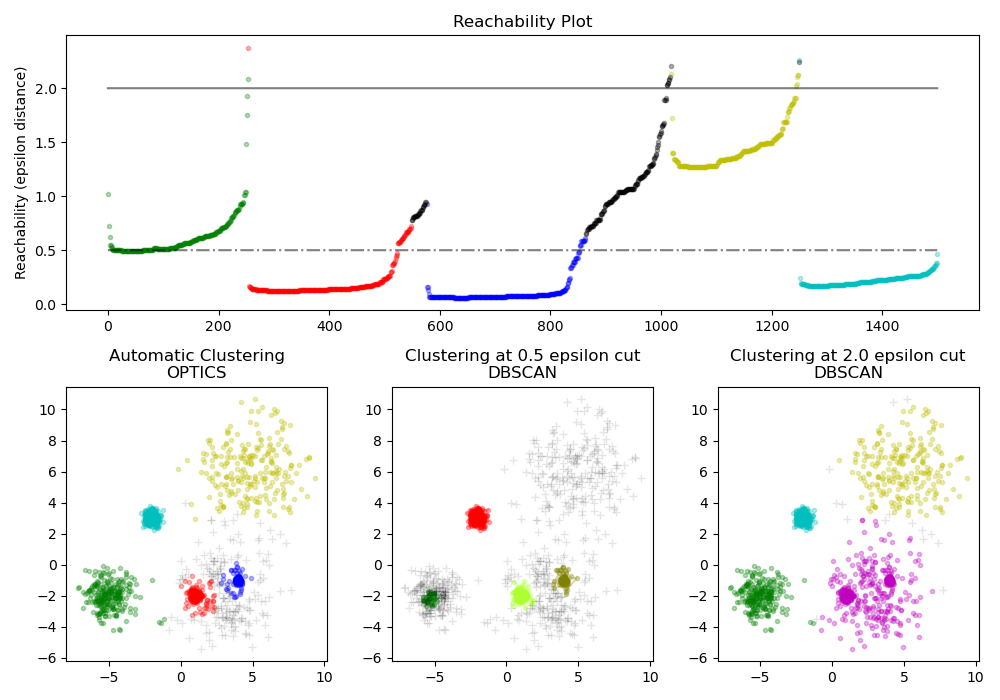
\includegraphics[width=0.9\linewidth]{figures/chapter3/sphx_glr_plot_optics_001.png}
  \caption{Reachability plot (above) of the exemplary dataset (row below). The reachability plot colouring was created for a $\xi$ \cite{10.1145/304182.304187} scheme of clustering. The first scatter plot in the second  row represents clustering for the Xi scheme as well. The next two plots are for epsilon cuts as specified in the plot's titles. (source: scikit-learn \cite{scikit-learn})}
  \label{fig:optics}
\end{figure}


